\documentclass[sigconf]{acmart}

\usepackage{booktabs} % For formal tables
\usepackage{algorithmicx}
\usepackage[ruled]{algorithm}
\usepackage{algpseudocode}
\usepackage{bold-extra}

\definecolor{stringColor}{rgb}{0.8,0.1,0.1}
\usepackage{listings}
\lstdefinelanguage{LF}{
  %keywords={typeof, new, true, false, catch, function, return, null, catch, switch, var, if, in, while, do, else, case, break},
  %more
  keywords={reaction, preamble, target, actor, composite, trigger, input, output, constructor, new, auto},
  keywordstyle=\color{black}\bfseries,
  ndkeywords={class, export, boolean, throw, implements, import, this},
  ndkeywordstyle=\color{darkgray}\bfseries,
  identifierstyle=\color{black},
  sensitive=false,
  comment=[l]{//},
  morecomment=[s]{/*}{*/},
  commentstyle=\color{purple}\ttfamily,
  stringstyle=\color{stringColor}\ttfamily,
  morestring=[b]',
  morestring=[b]"
}
\lstset{
   language=C,
   backgroundcolor=\color{white},
   extendedchars=true,
   basicstyle=\footnotesize\ttfamily,
   showstringspaces=false,
   showspaces=false,
   numbers=left,
   numberstyle=\tiny,
   numbersep=5pt,
   tabsize=2,
   breaklines=true,
   showtabs=false,
   captionpos=b,
   xleftmargin=7pt, xrightmargin=0pt
}

\newcounter{myctr}
\newenvironment{compactEnumerate}{\begin{list}{\arabic{myctr}.}
{\usecounter{myctr}
%\setlength{\topsep}{1mm}\setlength{\itemsep}{0.5mm}
\setlength{\topsep}{0.3mm}\setlength{\itemsep}{0mm}
\setlength{\parsep}{0.3mm}
\setlength{\itemindent}{0mm}\setlength{\partopsep}{0mm}
\setlength{\labelwidth}{15mm}
\setlength{\leftmargin}{4mm}}}{\end{list}}

% Copyright
%\setcopyright{none}
\setcopyright{acmcopyright}
%\setcopyright{acmlicensed}
%\setcopyright{rightsretained}
%\setcopyright{usgov}
%\setcopyright{usgovmixed}
%\setcopyright{cagov}
%\setcopyright{cagovmixed}


\copyrightyear{2019} 
\acmYear{2019} 
%\setcopyright{acmlicensed}
\acmConference[DAC '19]{The 56th ACM/ESDA/IEEE Design Automation Conference}{June 2--6, 2019}{Las Vegas, USA}
%\acmBooktitle{The 34th ACM/SIGAPP Symposium on Applied Computing (SAC '19), April 8--12, 2019, Limassol, Cyprus}
%\acmPrice{15.00}
%\acmDOI{10.1145/3297280.3297337}
%\acmISBN{978-1-4503-5933-7/19/04}



%\acmArticle{4}
%\acmPrice{15.00}

% These commands are optional
%\acmBooktitle{Transactions of the ACM Woodstock conference}
%\editor{Jennifer B. Sartor}
%\editor{Theo D'Hondt}
%\editor{Wolfgang De Meuter}

%%%%%%%%%%%%%%%%%%%%%%%%%%%%%%%%%%%%%%%%%%%%%%%%%%%%

\usepackage{amsmath}
\usepackage{amssymb}
\usepackage{subcaption}
\usepackage{multicol}
\usepackage[inline]{enumitem}
\usepackage{xcolor} 
\usepackage{ifthen}


%%%%%%%%%%%%%%%%%%%%%%%%%%%%%%%%%%%%%%%%%%%%%%%%%%%%
% Note style by Sebastian Ertel
%%%%%%%%%%%%%%%%%%%%%%%%%%%%%%%%%%%%%%%%%%%%%%%%%%%%

\newboolean{showcomments}
\setboolean{showcomments}{true} %set false for final submission
\ifthenelse{\boolean{showcomments}}
{ \newcommand{\mynote}[3]{
   \fbox{\bfseries\sffamily\scriptsize#1}
   {\small$\blacktriangleright$\textsf{\emph{\color{#3}{#2}}}$\blacktriangleleft$}}}
{ \newcommand{\mynote}[3]{}}
\definecolor{asparagus}{rgb}{0.53, 0.66, 0.42}

% One command per author:
\newcommand{\todo}[1]{\mynote{TODO}{#1}{red}}
\newcommand{\martin}[1]{\mynote{Martin}{#1}{blue}}% 
\newcommand{\marten}[1]{\mynote{Marten}{#1}{cyan}}% 
\newcommand{\isa}[1]{\mynote{Isabelle}{#1}{darkgreen}}% 
\newcommand{\ag}[1]{\mynote{Andr\'es}{#1}{asparagus}}% 
\newcommand{\armin}[1]{\mynote{Armin}{#1}{purple}}%
\newcommand{\marjan}[1]{\mynote{Marjan}{#1}{magenta}}% 
\newcommand{\edward}[1]{\mynote{Edward}{#1}{magenta}}% 

\newcommand{\keyword}[1]{\texttt{\textbf{#1}}}
\begin{document}

\title{Actors, Timestamps, and Determinism for Time-Critical Systems}


\author{Marten Lohstroh}
\orcid{0000-0001-8833-4117}
\email{marten@eecs.berkeley.edu}
% \affiliation{%
% 	\institution{University of California, Berkeley}
% 	%\streetaddress{}
% 	%\postcode{}
% 	%\city{} 
% 	\country{USA} 
% }

\affiliation{%
	\institution{UC Berkeley, USA}
	%\streetaddress{}
	%\postcode{}
	%\city{} 
	% \country{USA} 
}

\author{Martin Schoeberl}
\orcid{1234-5678-9012}
\email{masca@dtu.dk}
\affiliation{%
	\institution{TU Denmark, Denmark}
	%\streetaddress{}
	%\postcode{2800}
	%\city{Lyngby} 
	% \country{Denmark} 
}

\author{Andr\'es Goens}
\orcid{}
\email{andres.goens@tu-dresden.de}
\affiliation{%
	\institution{TU Dresden, Germany}
	%\streetaddress{}
	%\postcode{}
	%\city{} 
	% \country{USA} 
}

\author{Armin Wasicek}
\orcid{}
\email{armin.wasicek@avast.com}
\affiliation{%
	\institution{Avast, USA}
	%\streetaddress{}
	%\postcode{}
	%\city{} 
	%\country{USA} 
}

\author{Christopher Gill}
\orcid{}
\email{cdgill@wustl.edu}

\affiliation{%
	\institution{Washington Univ., St. Louis, USA}
	%\streetaddress{}
	%\postcode{}
	%\city{} 
	%\country{USA} 
}

\author{Marjan Sirjani}
\orcid{}
\email{marjan.sirjani@mdh.se}

\affiliation{%
	\institution{M\"alardalen Univ., Sweden}
	%\streetaddress{}
	%\postcode{}
	%\city{} 
	%\country{Sweden} 
}

\author{Edward A. Lee}
\orcid{0000-0002-5663-0584}
\email{eal@eecs.berkeley.edu}

\affiliation{%
	\institution{UC Berkeley, USA}
	%\streetaddress{}
	%\postcode{}
	%\city{} 
	%\country{USA} 
}


\renewcommand{\shortauthors}{M. Lohstroh et al.}

\begin{abstract}
Programming time-critical systems is notoriously difficult, since it requires precise control over both the computational and timing aspects of the system behavior. In this paper we propose a programming model aimed at these systems. 
Oriented on actors, our model reduces nondeterminism using has a semantic notion of time centered around timestamps.
This allows programmers to specify timing properties and ensures that messages between actors are handled in deterministic order unless nondeterminism is introduced explicitly as a desired property.
\end{abstract}

%
% The code below should be generated by the tool at
% http://dl.acm.org/ccs.cfm
% Please copy and paste the code instead of the example below. 
%
\begin{CCSXML}
	<ccs2012>
	<concept>
	<concept_id>10010520.10010553.10010562</concept_id>
	<concept_desc>Computer systems organization~Embedded systems</concept_desc>
	<concept_significance>500</concept_significance>
	</concept>
	</ccs2012>  
\end{CCSXML}

\ccsdesc[500]{Computer systems organization~Embedded systems}


\keywords{actor, real-time systems, worst-case execution time}

\maketitle

\section{Introduction}\label{sec:intro}
Precision timing plays an important role in a plethora of modern systems, ranging anywhere from embedded control systems that continually interact with concurrent physical processes (i.e., cyber-physical systems) to large-scale distributed systems requiring some measure of consistency.
In order to effectively program these systems, there is a need for programming models with semantics that include time.
In current-day general-purpose hardware and programming languages, timing properties of software are emergent rather than specified.
Therefore, the verification of timing properties of time-critical systems relies on testing, but effectively testing software in the face of nondeterminism is challenging.

In this paper, we propose an actor-oriented programming model aimed at time-critical systems. This model reduces nondeterminism by introducing a semantic notion of time, allowing programmers to specify timing properties, which, if executed on capable hardware, can be guaranteed statically. The coordination semantics, based on discrete events, ensure that messages between actors are handled in deterministic order unless nondeterminism is introduced explicitly as a desired property.

\section{Actors}\label{sec:actor}
The actor model was introduced by Hewitt~\cite{DBLP:conf/ijcai/HewittBS73} in the early 70s. 
%A well-known programming paradigm used in this context are Hewitt~\cite{Hewitt:77:Actors} actors.
Since then,
%their introduction in the 70s,
%NOTE: removed citation of Scala (haller2009scala)
the use of actors has proliferated in programming languages~\cite{Armstrong:96:Erlang,desai2013p}, coordination languages~\cite{ren1995rtsynchronizer,ARC}, distributed systems~\cite{Hunt2018, DBLP:journals/corr/abs-1712-05889}, 
and simulation engines~\cite{Ptolemy:14:Book,DBLP:journals/fuin/SirjaniMSB04}. 
%\ag{In case we need space: here we can certainly remove a citation or two.}
Actors have much in common with objects---a paradigm focused on reducing code replication by means of inheritance and increasing modularity via data encapsulation---but unlike objects, actors provide a better model for \emph{concurrency} than threads, the default model for objects.
Indeed, each actor is presumed to operate concurrently alongside other actors with which it may exchange messages asynchronously. 
Objects, in contrast, are usually designed assuming a single thread of control, and retrofitting them to be ``thread safe'' is challenging and error prone.
The inherent concurrency of actors makes them ideal for programming reactive systems.
However, the lack of any guarantees with respect to the ordering of messages and the absence of a notion of time make this 
model less useful for specifying systems in which timely execution and repeatable behavior are important.

\subsection{Verifiable Timing}\label{sec:related}
Extra machinery can be introduced for the formal specification and analysis of systems composed of Hewitt actors.
For instance, Real-time Maude~\cite{olveczky:2008:real}, a timed rewriting logic framework and temporal model checking tool, has been applied to actors in~\cite{Ding2003}.
Similarly, the modeling language Rebeca performs analysis that uses a model checker to ensure that nondeterminism allowed in the model does not lead to behaviors that violate timing requirements~\cite{KHAMESPANAH2015184}.
%\cite{DBLP:conf/birthday/SirjaniJ11}.
%\marjan{, and for the timed version in \cite{KHAMESPANAH2015184}.}\marten{I would prefer to cite [102], [103], or [104] from \cite{DBLP:conf/birthday/SirjaniJ11} rather than \cite{DBLP:conf/birthday/SirjaniJ11} itself (it is a survey paper). I chose \cite{KHAMESPANAH2015184} because it is the most recent paper I could find that technically discusses the approach.}
%\marjan{Okay, I understand, \cite{KHAMESPANAH2015184} is a good ref. for Timed Rebeca, and timed actors.  \cite{DBLP:conf/birthday/SirjaniJ11} is about anayzing actors with no timing feature. }
Alternatively, constraints can be placed on actors' allowable behaviors so that they adhere to a well-defined model of computation (MoC), satisfying desirable properties such as deadlock freedom, schedulability, bounded memory usage, and deterministic execution, by construction. It is the latter approach that we follow.

In \cite{ren1995rtsynchronizer}, Ren and Agha also propose giving actors a temporal
semantics. As in our work, they assume a sufficiently well synchronized
common physical time base shared by all actors, and they express timing
requirements as constraints on message handling. Their work differs from
ours, however, in that they build off a standard actor language, thereby
inheriting its nondeterministic ordering of message handling, and they
rely on separately imposing timing constraints to control the order when
needed. In contrast, we use logical timestamps to define the order of
message handling and ensure determinism.

Dataflow models are also closely related to the actor approach. In~\cite{wiik2018contract} the authors extend an (untimed) dataflow model with formal contracts that allow guarantees, e.g., for scheduling.
There are timed models of dataflow~\cite{Sriram:00:Scheduling}, and even some structured approaches to use timing semantics in dataflow to execute time-critical applications in cyber-physical systems~\cite{GeilenEtAl:12:Scenarios}.
%These models are more restrictive than our proposed work and lack the polyglot flexibility of our approach.

Fredlund et al. proposed timed extension of McErlang
as a model checker of timed Erlang programs in \cite{DBLP:conf/forte/EarleF12}. In this extension a new API is introduced to provide the definition and manipulation of timestamps.
%In \cite{DBLP:journals/csur/BoerSHHRDJSKFY17}, de Boer et al. provided a survey on active object languages but there is no focus on timed features.

% \todo{As discussed in call: do we need these?}
% Towards a real-time coordination model for mobile computing \cite{hackmann2005towards}
% Method and tools for mixed-criticality real-time applications within PharOS \cite{lemerre2011method}
% Accessors \cite{brooks2018component}
% S-Net~\cite{grelck2008gentle}
% Guarded Atomic Actions~\cite{Rosenband:2004:MSG:996566.996583}
% Timed C \cite{Broman_timedC}

\subsection{Reactors, Informally}

The approach we describe in this paper replaces classical actors with a model that we call ``reactors,''
which are similar to actors, but with important differences.
We will explain the model first, and then discuss its advantages.
We do not make a commitment to a specific syntax for specifying reactors,
but, to be concrete, we show in Figure \ref{fig:code} one possible syntax
and specific simple application.

\begin{figure}[ht]
\centering
\begin{minipage}{0.50\linewidth}
\begin{lstlisting}[language=LF]
target C;
reactor Ramp(p:int(10)) {
	output out:int;
	clock c(p);
	constructor {=
		int count = 0;
	=}
	reaction(c) -> out {=
		count++;
		set(out, count);
	=}
}
\end{lstlisting}
\end{minipage}%
\begin{minipage}{0.45\linewidth}
\begin{lstlisting}[language=LF,firstnumber=13]

reactor Print {
	input in:int;
	reaction(in) {=
		printf("%d\n", in);
	=}
}
composite App {
	a = new Ramp(prd=100);
	b = new Print();
	a.out -> b.in;
}
\end{lstlisting}
\end{minipage}
 \caption{\keyword{Ramp} feeding into a \keyword{Print} actor}
 \label{fig:code}
\end{figure}

\edward{Informal description of the example}

Reactors can also be used to handle less predictable asynchronous behaviors,
such as network interactions, interrupt-driven sporadic sensors, and other unpredictable events.
A simple example is sketched in Figure \ref{fig:async}.
That example is an reactor with a single input, \texttt{url}.
\edward{Informal description of the example}


\begin{figure}[ht]
\begin{lstlisting}[language=LF]
reactor REST() {
	input url:string;
	output out:string;
	action arrival:string;
	reaction(url) --> arrival {=
		httpRequest(url, function(reply) {
			schedule(arrival, reply);
		});
	=}
	reaction(arrival) -> out {=
		set(out, arrival);
	=}
}
\end{lstlisting}
 \caption{Example of a reactor that produces an asynchronous output.}
 \label{fig:async}
\end{figure}

\subsection{Reactor Principles}

We summarize our model in terms of the following principles.

\paragraph{Actors and Message Exchange}
\begin{enumerate}
	\item Actors have input ports, triggers, output ports, state, and an ordered list of reactions.
	\item Each actor operates in the context of a composite (i.e., an actor that contains other actors), which manages connections between actors, the delivery of messages, and the scheduling and execution of reactions;
	\item A message is sent via a port, and it is delivered to the ports of other actors via a connection; a port must be connected to the port of another actor within the same composite before it can receive messages.
	\item An actor may send messages to multiple input ports or multiple actors;
	these messages all bear the same timestamp.
	\item No two distinct actors may send messages to the same input port of another actor;
	a composition of actors that allows this is erroneous.
	\item Messages sent/received by actors are timestamped and denote a discrete event.
\end{enumerate}

\paragraph{Reactions}
\begin{enumerate}
	\setcounter{enumi}{6}
	\item A reaction is a procedure, and any two reactions of an actor are mutually exclusive; they execute atomically with respect to one another.
	\item A reaction can read and modify the actor's state.
	\item Reactions can not be directly invoked by actors themselves (or by other actors).
	\item Each reaction declares the input ports and triggers to which it reacts and to which output ports it may write.
	\item At a logical time, a reaction may read inputs that are not triggering inputs, but it must declare that it reads those inputs, and those inputs may be \emph{absent} (no event is present at this logical time).
	\item If a reaction declares that it reacts to multiple input ports, then at the time of the reaction, at least one of those
	input ports will have a message time-stamped with the time of the reaction, but the other input ports may be \emph{absent}
	(no event is present at this logical time).
	\item A reaction can set the values of the output ports that is it has declared, and if it does so, a message will be sent after the conclusion of the reaction with a payload equal to the final value set by the reaction.
	\item If multiple reactions write to the same output port, then the message sent will be that set by the last reaction invoked. \ag{Why? Isn't this unintuitive? Why not have all messages sent (e.g. with the same timestamp and superdense ordering in the execution order of the producing reactions)?}
	\item A reaction can schedule a trigger at a future logical time.
\end{enumerate}

\paragraph{Passage of Logical Time}
\begin{enumerate}
	\setcounter{enumi}{16}
	\item At each logical time for which there is an input message or trigger, all reactions to those inputs and triggers will be invoked in the order in which the reactions are defined. \ag{At this points the signals are consumed, right? I would say this explicitly}
	\item Logical time is constant during execution of a reaction.
	\item For each reaction, logical time is strictly increasing; that is, a reaction will never be invoked at a logical time that is equal to or less than that of a previous invocation.
\end{enumerate}


%\begin{enumerate}
%\item Messages exchanged between actors are timestamped and denote a discrete event.
%\item Actors have input ports, triggers, output ports, state, and an ordered list of reactions.
%\item A reaction is a procedure, and any two reactions of an actor are mutually exclusive; they execute atomically with respect to one another;
% \item Each reaction declares the input ports and triggers to which it reacts and to which output ports it may write.
% \item If a reaction declares that it reacts to multiple input ports, then at the time of the reaction, at least one of those
% input ports will have a message time-stamped with the time of the reaction, but the other input ports may be \emph{absent}
% (no event is present at this logical time).
% \item A reaction must also declare inputs that it does not react to but that it reads;
% at a logical time, those inputs may also be absent.
% \item At each logical time for which there is an input message or trigger, all reactions to those inputs and triggers will be invoked in the order in which the reactions are defined.
% \item Logical time is constant during execution of a reaction.
% \item For each reaction, logical time is strictly increasing; that is, a reaction will never be invoked at a logical time that is equal to or less than that of a previous invocation.
% \item A reaction can schedule a trigger at a future logical time.
% \item A reaction can read and modify the actor's state.
%  \item A reaction can set the values of the output ports that is it has declared, and if it does so, a message will be sent after the conclusion
% of the reaction with a payload equal to the final value set by the reaction.
% \item If multiple reactions write to the same output port, then the message sent will be that set by the last reaction invoked.
% \item No two distinct actors may send messages to the same input port of another actor;
% a composition of actors that does this is an erroneous composition.
% \item An output port may send messages to multiple input ports or multiple actors;
% these messages all bear the same timestamp.
% % \edward{Note that this has dependency implications... An output message cannot be sent until the last reaction declaring that output has had a chance to run.}
% \item At a logical time, a reaction may read inputs that are not triggering inputs, but it must declare that it reads those inputs,
% and those inputs may be \emph{absent} (no event is present at this logical time).
% \item \martin{We are not talking about delay here, but logical time is constant during reaction. There is no explicit
% mentioning that the output timestamp is the same as the input timestamp (except when having a delay on
% a reaction).}\marten{If we implement Delay using an actor that self-schedules a delayed reaction, the claim that no time passes during a reaction still holds.}
%\end{enumerate}

Together, these rules ensure that the execution of a composition of actors is deterministic
in the sense that given any set of time-stamped inputs from outside the composition, the composition has exactly one behavior.
This determinism can be proved by showing that at each logical time, every actor realizes a monotonic function in an appropriately
chosen partial order and that the execution converges to a least fixed point in this partial order~\cite{LeeZheng:07:SRDECT}.
Within these rules, there are various opportunities for ``syntactic sugar,'' where complex behaviors can be expressed
more compactly, for example with the Ptolemy II notion of ``multiports'' or ``persistent ports'' \cite{Ptolemy:14:Book}.

%\martin{ We have discussed two different input ports:
%those that are only valid during the logical time of the timestamp (what did we call them?)
%and the ones that latch the value and are valid in future logical time as well.}
%\marten{I think we called them input ports and triggers, respectively. See item (3)(a). If unclear, we should definitely improve the wording. Same for the terminology. We could also go for external/internal input ports. Internal ports are only referenced by the actor itself; both can be considered triggers...}
%\martin{I don't think this is trigger. An input port may be part of a trigger, and for the ones that are only valid
%during the local time need to be part of a trigger condition. Otherwise they would not make any sense.
%The discussion came on what is the meaning when a reaction uses two inputs, but only one is
%triggering it. What is the value of the other: either absent or the last value (the latching input).
%That latching input needs a default value. And that is actually the way to specify it in the accessors
%framework (according to Edward, I have not checked).}
%\marjan{So, do we have two types of ports? one can only accept "events" and other can only accept "values"?}
%\martin{Both types are ``events'' with a timestamp that can trigger a reaction. The question is when
%a port is read that has not an event with the current logical time: is the content just ``absent'' or does it
%have the ``last seen'' value. I think both might be useful. Although it is probably syntactic sugar.
%The latching port can be simulated by a trigger on the input and storing the value in the state of
%the actor. Maybe this would be a leaner and cleaner semantic.}
%\marjan{Ok, I think I understand what you mean. And I am just thinking, sometimes we need to know if the event at the other port is "new" or not too old, can we do that here? I guess we can write a code for that, keeping the "model timestamp" of the "last seen" value maybe ... }






\subsection{Discussion}

In the original Hewitt actors and many modern implementations, actors have references to the actors that they communicate with.
In our approach, rather than addressing each other directly, actors exchange messages via ports. This level of indirection allows actors to be agnostic to the presence or absence of their counterparts. The connections between actors are embedded in a level of hierarchy---a composite---that is responsible for transporting messages between contained actors. This approach increases modularity and, more importantly, exposes dependencies between actors.

All messages communicated between actors in our model are timestamped. Message exchange is coordinated under a discrete-event (DE) semantics \cite{LeeEtAl:7:DiscreteEvents}, which guarantees that actors observe messages in timestamp order.
DE semantics is formally rooted in that of synchronous/reactive MoCs~\cite{LeeZheng:07:SRDECT}, to increase efficiency, we avoid performing a fixed-point computation by executing actors in topological order. That way, each actor is only executed at most once per tick of the logical clock. The schedule for message delivery is based purely on the topology of the actor graph.
%, and no static analysis of the actors' internals is required. 
%---the actors are treated as black boxes. 
Dynamic changes in the topology are handled hierarchically, so that the extent of the graph that is subject to rescheduling is contained when reconfigurations occur during runtime. A runtime reconfiguration always occurs within a composite actor that can coordinate it in a predictable and orderly fashion. %whose interface remains unchanged.\marten{This is not completely true. I/O dependencies may change, which may lead to scheduling problems outside of the composite. The good thing is that we can detect problems before enacting the changes, but it could potentially require communication with composites up the hierarchy.} 

Actors are useful for encapsulating state, though it is often necessary for distinct but related computational activities to share state. For instance, a single actor to could serve as a proxy for a device (e.g, a hub for smart lights), for which it performs several different tasks.
Integrating related activities into a single atomic actor with multiple ports improves performance and hides complexity, but we do not want to obscure internal dependencies between inputs and outputs that could inform the schedule for message delivery. Without it, for instance, the scheduler has to conservatively assume that \emph{any} output of an actor depends on \emph{all} of its inputs, and reject configurations that could introduce zero-delay feedback. Causality interfaces~\cite{ZhouLee:08:CausalityInterfaces} can be used to make dependencies visible at the interface level. Rather than relying on annotations that could potentially be unsound, or inferring them via static code analysis, we propose to make causality interfaces an integral part actor definitions. Specifically, this can be done by breaking an actor's functionality down into \emph{reactions}, each of which is subject to simple lexical scoping rules that limit its access to the actors' input and output ports, thereby eliminating dependencies between ports that are out of scope.


The functionality of a reaction can be treated as a black box; a schedule can be devised purely base on dependency information. This very feature opens the possibility for a \emph{polyglot} language design. We can mix interface definitions and composition primitives with target language code that implements the functionality of the actors. A major advantage of this approach is that our programming model can target anything from the most primitive, resource constrained, deeply embedded systems to highly dynamic distributed systems. 

%Consider the following example of what such a polyglot actor definition could look like:
% also, no need for postfire % maybe mention that this optimization comes at the loss of the ability of handling some zero-delay feedback models...

% The first reaction is triggered by events on the {\tt apply} port; it applies the brakes when the received value is above a threshold, and sets the state (brake pressed or not) accordingly; no outputs are produced by this reaction. The second reaction, triggered by events on the {\tt check} port, simply reports the current state of the actor. To ensure determinism, if {\tt apply} and {\tt check} receive an event simultaneously (i.e., the timestamps associated with the events are equal), the reactions will be triggered in order of declaration. Each reaction runs until completion before the next reaction is triggered.

For example, actors might be defined and composed as shown in Fig.~\ref{fig:code}. The first line specifies that the target language is C. The second line defines an \keyword{actor} named {\tt Source} with a parameter named {\tt p} that has type {\tt int} and default value {\tt 10}. This actor also has an \keyword{output} named {\tt out}. A \keyword{trigger} is like an input port in that it receives messages, but it is ``private'' in the sense that it receives only messages initiated by its own actor. The statement on line 4 indicates that an event is expected to automatically appear at {\tt t}\ag{I don't understand this sentence.}. The first argument passed to the \keyword{trigger} indicates a zero time offset for the arrival of the first event, and the second argument indicates the event should reoccur with a time period {\tt p}. On line 5, a \keyword{constructor} delimits the first block of C code that is used to declare variables and functions that may be referenced in any of the actor's reactions. All target code is delimited by {\tt \{=} and {\tt =\}}.
A \keyword{reaction} (lines 8, 16) declares the inputs or triggers that cause it to execute between braces.
Outputs that it may set are listed after.
If the \keyword{reaction} had additional inputs or triggers that it might use, these would be listed before the {\tt ->}. \ag{perhaps actually add to the example or remove this sentence completely? It's probably not necessary.}
Finally, the \keyword{composite} declared on line 20 instantiates a {\tt Ramp} and {\tt Print} actors and connects them (line 23). 
\marten{Not yet happy about the flow of the above paragraph.}
\ag{I'd question more if we need the whole paragraph (and the example), because we're not actually presenting any concrete syntax here now. Perhaps we should remove it.}


\section{Coordination Semantics}


% Sort reactions topologically based on precedences.

% Global notion of “current time” t.

% Event queue containing future events.

% Choose earliest timestamp t’ on the queue.

% Wait for the real-time clock to match t’.

% Execute actors in topological sort order.

% \begin{figure}[ht]
% \begin{algorithmic}[1]
%  \Procedure{execute}{}
   
%  \EndProcedure
%  \end{algorithmic}
% \caption{The Lingua Franca execution engine \marten{Maybe too much detail}}
% \label{fig:lf-engine}
% \end{figure}

% Time is \emph{logical} time. This logical time be used for simulation and then
% we call it model time. We can also use the network of actors for the implementation
% of the system. 

% In that case wall clock time is used to timestamp input values
% at sensors. Logical time can never advance further than wall clock time.
% We have a notion of delay in two places: (1) as a delay actor to break up
% feedback loops (2) at actuators to specify that an actuation shall happen before
% (or exactly at) the logical time of the input plus the delay.

% Actors communicate via ports. All data exchanged has a timestamp.
% An actor does not advance time, the reaction is considered instantaneous.

% Reactions of one actor are atomic and are allowed to change state.
% Reactions are triggered by available inputs with timestamps at logical
% time (or older). When several reactions of an actor are enabled at the
% same time, the definition order in LF defines the execution order.

% A reaction of an actor can also be released by a trigger. A trigger
% can be periodic triggers or a single shot timer.
%The engine that drives the execution of LF actors (see Figure~\ref{fig:lf-engine}) enforces the following principles:

% \subsection{Compiler Tool Chain}

% \begin{figure}[ht]
%  \centering
%  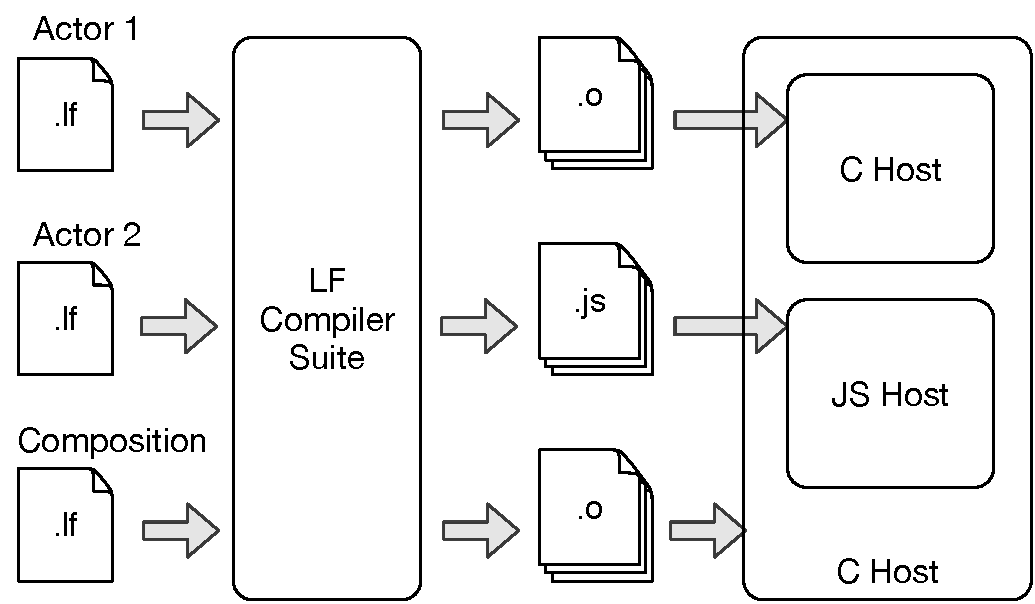
\includegraphics[width=0.8\linewidth]{img/lf-compiler}
%  \caption{The Envisioned Tool Chain}
%  \label{fig:lf-compiler}
% \end{figure}

% For Lingua Franca we envision a tool chain as depicted in Figure~\ref{fig:lf-compiler}.
% Code will first be parsed for the LF semantics, producing object files or code specific to the used language and host targeted.
% Analysis such as semantic soundness or timing guarantees when permitted can be included as part of this LF compiler suite.
% Different actors are integrated as composites in a (logically) distinct host.
% \ag{this is my (perhaps outdated) understanding of the envisioned tool chain. Feel free to change this and/or ask for changes in the Figure.}

% Time is \emph{logical} time. This logical time be used for simulation and then
% we call it model time. We can also use the network of actors for the implementation
% of the system. In that case wall clock time is used to timestamp input values
% at sensors. Logical time can never advance further than wall clock time. \marten{Not entirely true: an optimized scheduler can do this under very specific circumstances that we'll elaborate on in the example.}


% The scheduler invokes reactions of actors dependent in inputs with timestamps
% that are equal (or earlier--can this happen?) at logical time $t_1$.
% Logical time cannot advance further than wall clock time $t_w$. If next logical
% time $t_2 > t_w$ the scheduler waits till $t_w \ge t_2$.

For dynamic systems, e.g., an IoT that keeps running, but in different contexts
(e.g., places), we support dynamic reconfiguration of the network of actors.
This may be well supported when targeting a dynamic language such as JavaScript,
but harder to implement in C.

To support runtime reconfiguration the target language needs access to actors and
ports. However, we can use scopes to having access to those parts of the framework
only in well defined places.

\martin{Will we talk about execution hosts such as PRET machines or Patmos
when targeting C and WCET analysis?}

\section{Time, Delays, and Deadlines}
Central to our programming model is the relationship between the timestamps of messages.
These timestamps denote \emph{logical} time, and the essential semantic feature is that every actor sees messages in time-stamp order.
When an actor receives multiple messages with the same timestamp, these messages are logically
\emph{simultaneous}, and the actor handles them in a well-defined deterministic order.
Logical time is distinct from \emph{physical time}, as measured anywhere in a networked application.
First, logical time remains constant during the execution of any reaction in any actor, and outputs produced by that reaction have
the same logical timestamp as the inputs that trigger the reaction.
\ag{Why do we do this? What would speak against having the timestamps of the output also be synchronized with physical time when sending them. I see more problems with having a logically instantaneous reaction than I see advantages with it.}
But if we establish a relationship between logical time and physical time, that can help to reliably deliver real-time behavior.

Consider the example in Fig.~\ref{fig:actor-graph}.



\todo{Explain delays )}
%SCRATCHPAD:
% We do not want to run ahead of realtime, because actors can produce spontaneous events that need to be stamped with 
% physical time, and we don't want these timestamps to be ``in the past.''
% The passing of \emph{physical} time is approximated by the system time of the execution platform. While logical time can be sped up or slowed down arbitrarily in a simulation, the fact that actors can interact with the physical world through sensors and actuators requires that logical time and physical time ``keep up'' with one another in order to have a temporal semantics that obeys the principle of causality (i.e., effects cannot precede causes) for all observers. 


% \subsection{Delays and Deadlines}

% We have a notion of delay in two places: (1) as a delay actor to break up
% feedback loops and (2) at actuators to specify that an actuation shall happen before
% (or exactly at) the logical time of the input plus the delay.

% Delays deserve also the purpose to align events with wall clock time and to
% allow execution of reactions in their worst-case execution time (WCET).
% The sum of all reaction's WCET from one synchronization point (either
% sample of sensors or output of a delay actor) to another synchronization
% point (or output of an actuator) has to be less than the delay.

\begin{figure}[ht]
 \centering
 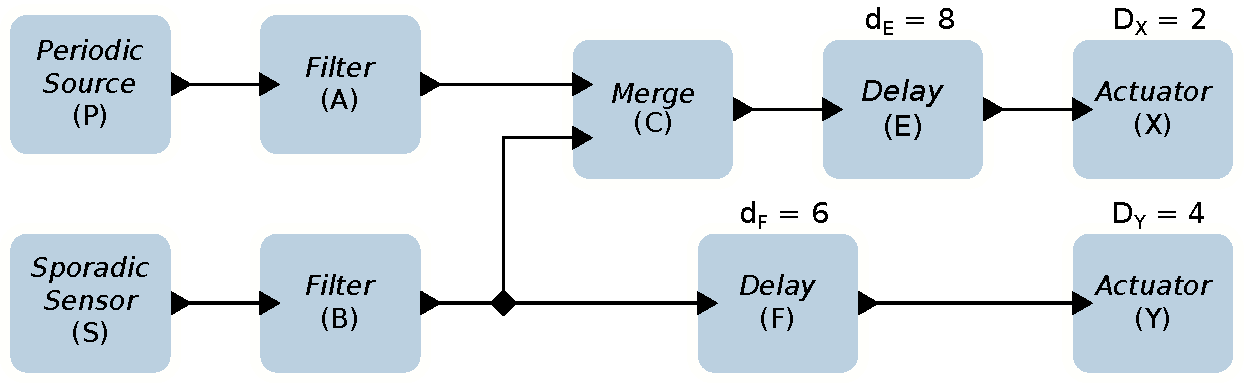
\includegraphics[width=\linewidth]{img/example}
 \caption{First example}
 \label{fig:actor-graph}
\end{figure}

While actors react in a coordinated fashion to messages from other actors, they could register an interrupt service routine or pass a callback to an asynchronous process that gets executed sporadically, bypassing the control of the composite. Any reaction that is expected to be triggered by such an event must be scheduled explicitly. The timestamp assigned to such reaction will be will be equal to the current physical time (i.e., obtained from a clock provided by the computation platform), provided that it is greater than the last seen (or current) logical time. 

% \marten{What do we do if there are events in the queue with a release time earlier than the current physical time? Let them go first? Or does the sporadic event go first?}
% Answer: Just assign the if our program is able to satisfy timing constraints, this situation will not occur.

\paragraph{Synchronization to Physical Time}
\begin{enumerate}
	\setcounter{enumi}{19}
	\item The logical time of any reaction that is scheduled inside an interrupt service routine or asynchronous callback (any computation that is not coordinated by the composite) will be equal to the current physical time (i.e., obtained from a clock provided by the computation platform). \todo{rephrase}
	\item \todo{Define the semantics of delays?}
\end{enumerate}
 

%This way, reactions can be triggered by asynchronous events without introducing possible race conditions with any on-going reactions.

% Sporadic events and call backs can trigger a reaction. This reaction is allowed
% to observe and also change the state of the actor. Therefore, they are not allowed
% to preempt a reaction (reactions are atomic to each other). To enforce this atomicity,
% a sporadic event 
%reaction is executed only between two logical timestamps $t_1$ and $t_2$.


\todo{Describe that the single threaded execution of JavaScript enforces
the restriction of the call back not interrupting the reaction.}
This can be enforced on a C based host by turning off interrupts when executing
a reaction. Interrupts are enabled when all
reactions for timestamp $t_1$ have been executed and disabled again when logical
time is advanced to $t_2$ where all reactions for $t_2$ are executed.

% \subsection{Causality}


% \begin{figure}[ht]
%  \centering
%  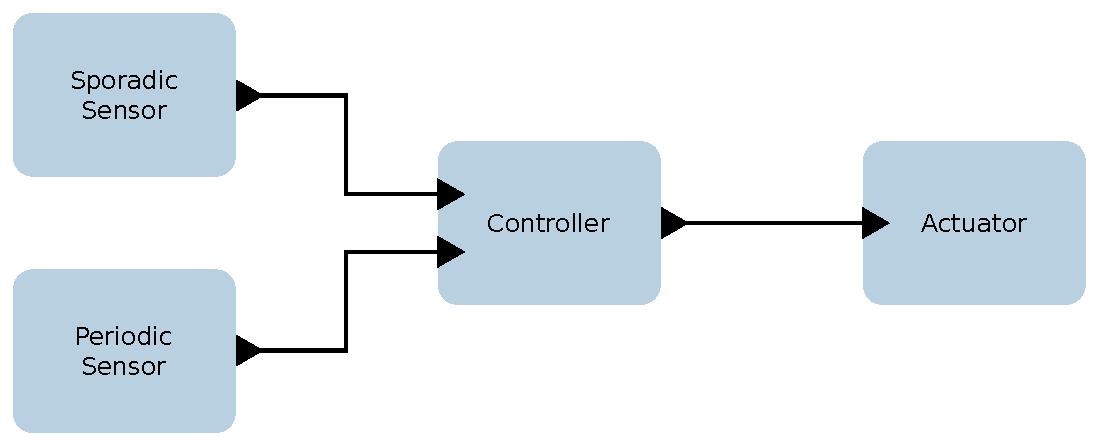
\includegraphics[width=\linewidth]{img/example-2}
%  \caption{Second example}
%  \label{fig:example-2}
% \end{figure}


% \subsection{Example 3}
% Shut off the lights some time after the switch has been flipped. Reason to have the deadline definition as stated: detectability. Suppose the start deadline cannot be met; the reaction should not be carried out (and the violation be reported on subsequently).

% \begin{figure}[ht]
%  \centering
%  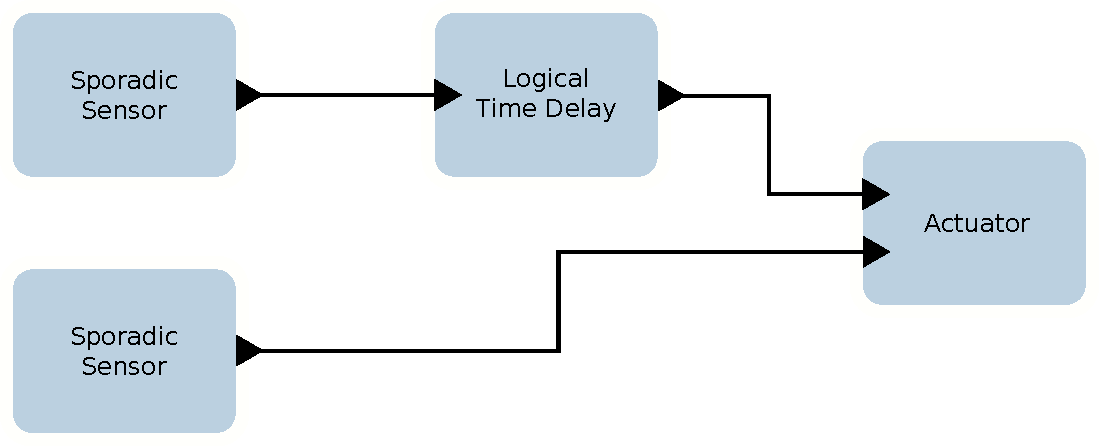
\includegraphics[width=\linewidth]{img/example-3}
%  \caption{Third example}
%  \label{fig:example-3}
% \end{figure}


%\section{Actors}
%


% Constraints can be placed on actors' allowable behaviors so that actors adhere to a well-defined model of computation, satisfying desirable properties such as deadlock freedom, schedulability, bounded memory usage, and deterministic execution by construction. This has been the guiding principle in the Ptolemy project\footnote{\url{https://ptolemy.berkeley.edu/}}, which studies modeling, simulation, and design of concurrent, real-time, embedded systems.

% Several frameworks have been built based, loosely or strictly, on the
% original Hewitt actor model
% \cite{Hewitt:77:Actors,Agha:97:ActorComputation}, including Akka
% \cite{AkkaAction2016},
% Ray \cite{DBLP:journals/corr/abs-1712-05889}, and Rebeca
% \cite{DBLP:journals/fuin/SirjaniMSB04}. One property of the original
% Hewitt actor model is that messages received by an actor from distinct
% sources are handled in nondeterministic order. \marten{even messages from the same source can arrive out-of-order}


% \martin{We need to check this: Outputs generated by a time triggered
% reaction are timestamped. When the system is simulated, the timestamp
% is equal to the model time. When the system is used for execution, the logical
% time for the release of the reaction is synchronized to wall clock time and therefore
% the output message are synchronized to wall clock time.}



% \martin{We have (and maybe support) two options: (1) input is only valid when
% the timestamp equals logical time, absent at other times or (2) keeping the value
% of an input for future logical time and having a default value for system initialization time.
% (in the JS accessors this is the way it is specified, the default value gives the
% ``keep'' or persistent semantic).}


\section{Conclusions}
\label{sec:conclusion}


\subsection*{Acknowledgments}
The work in this paper was supported in part by the National Science Foundation (NSF),
award \#CNS-1836601 (Reconciling Safety with the Internet) and the iCyPhy Research Center
(Industrial Cyber-Physical Systems, supported by Avast, Camozzi Industries, Denso, Ford, Siemens, and Toyota
This  work  was also supported in part by the Center for Advancing Electronics Dresden (cfaed) and the German Academic Exchange Service (DAAD). 

\bibliographystyle{ACM-Reference-Format}
\bibliography{Refs} 

\end{document}
